\counterwithin{table}{section}

\newpage

% Set section counter to 5
\setcounter{section}{5}
\renewcommand\thesection{\arabic{section}}
\renewcommand\thesubsection{\arabic{subsection}}

\label{lampiran1}
\begin{center}
    \phantomsection
    \addcontentsline{toc}{section}{LAMPIRAN I SURAT KETERANGAN}
    \section*{\textbf{LAMPIRAN I SURAT KETERANGAN}}
\end{center}
            \begin{secondfigure}[H]
                \centering
                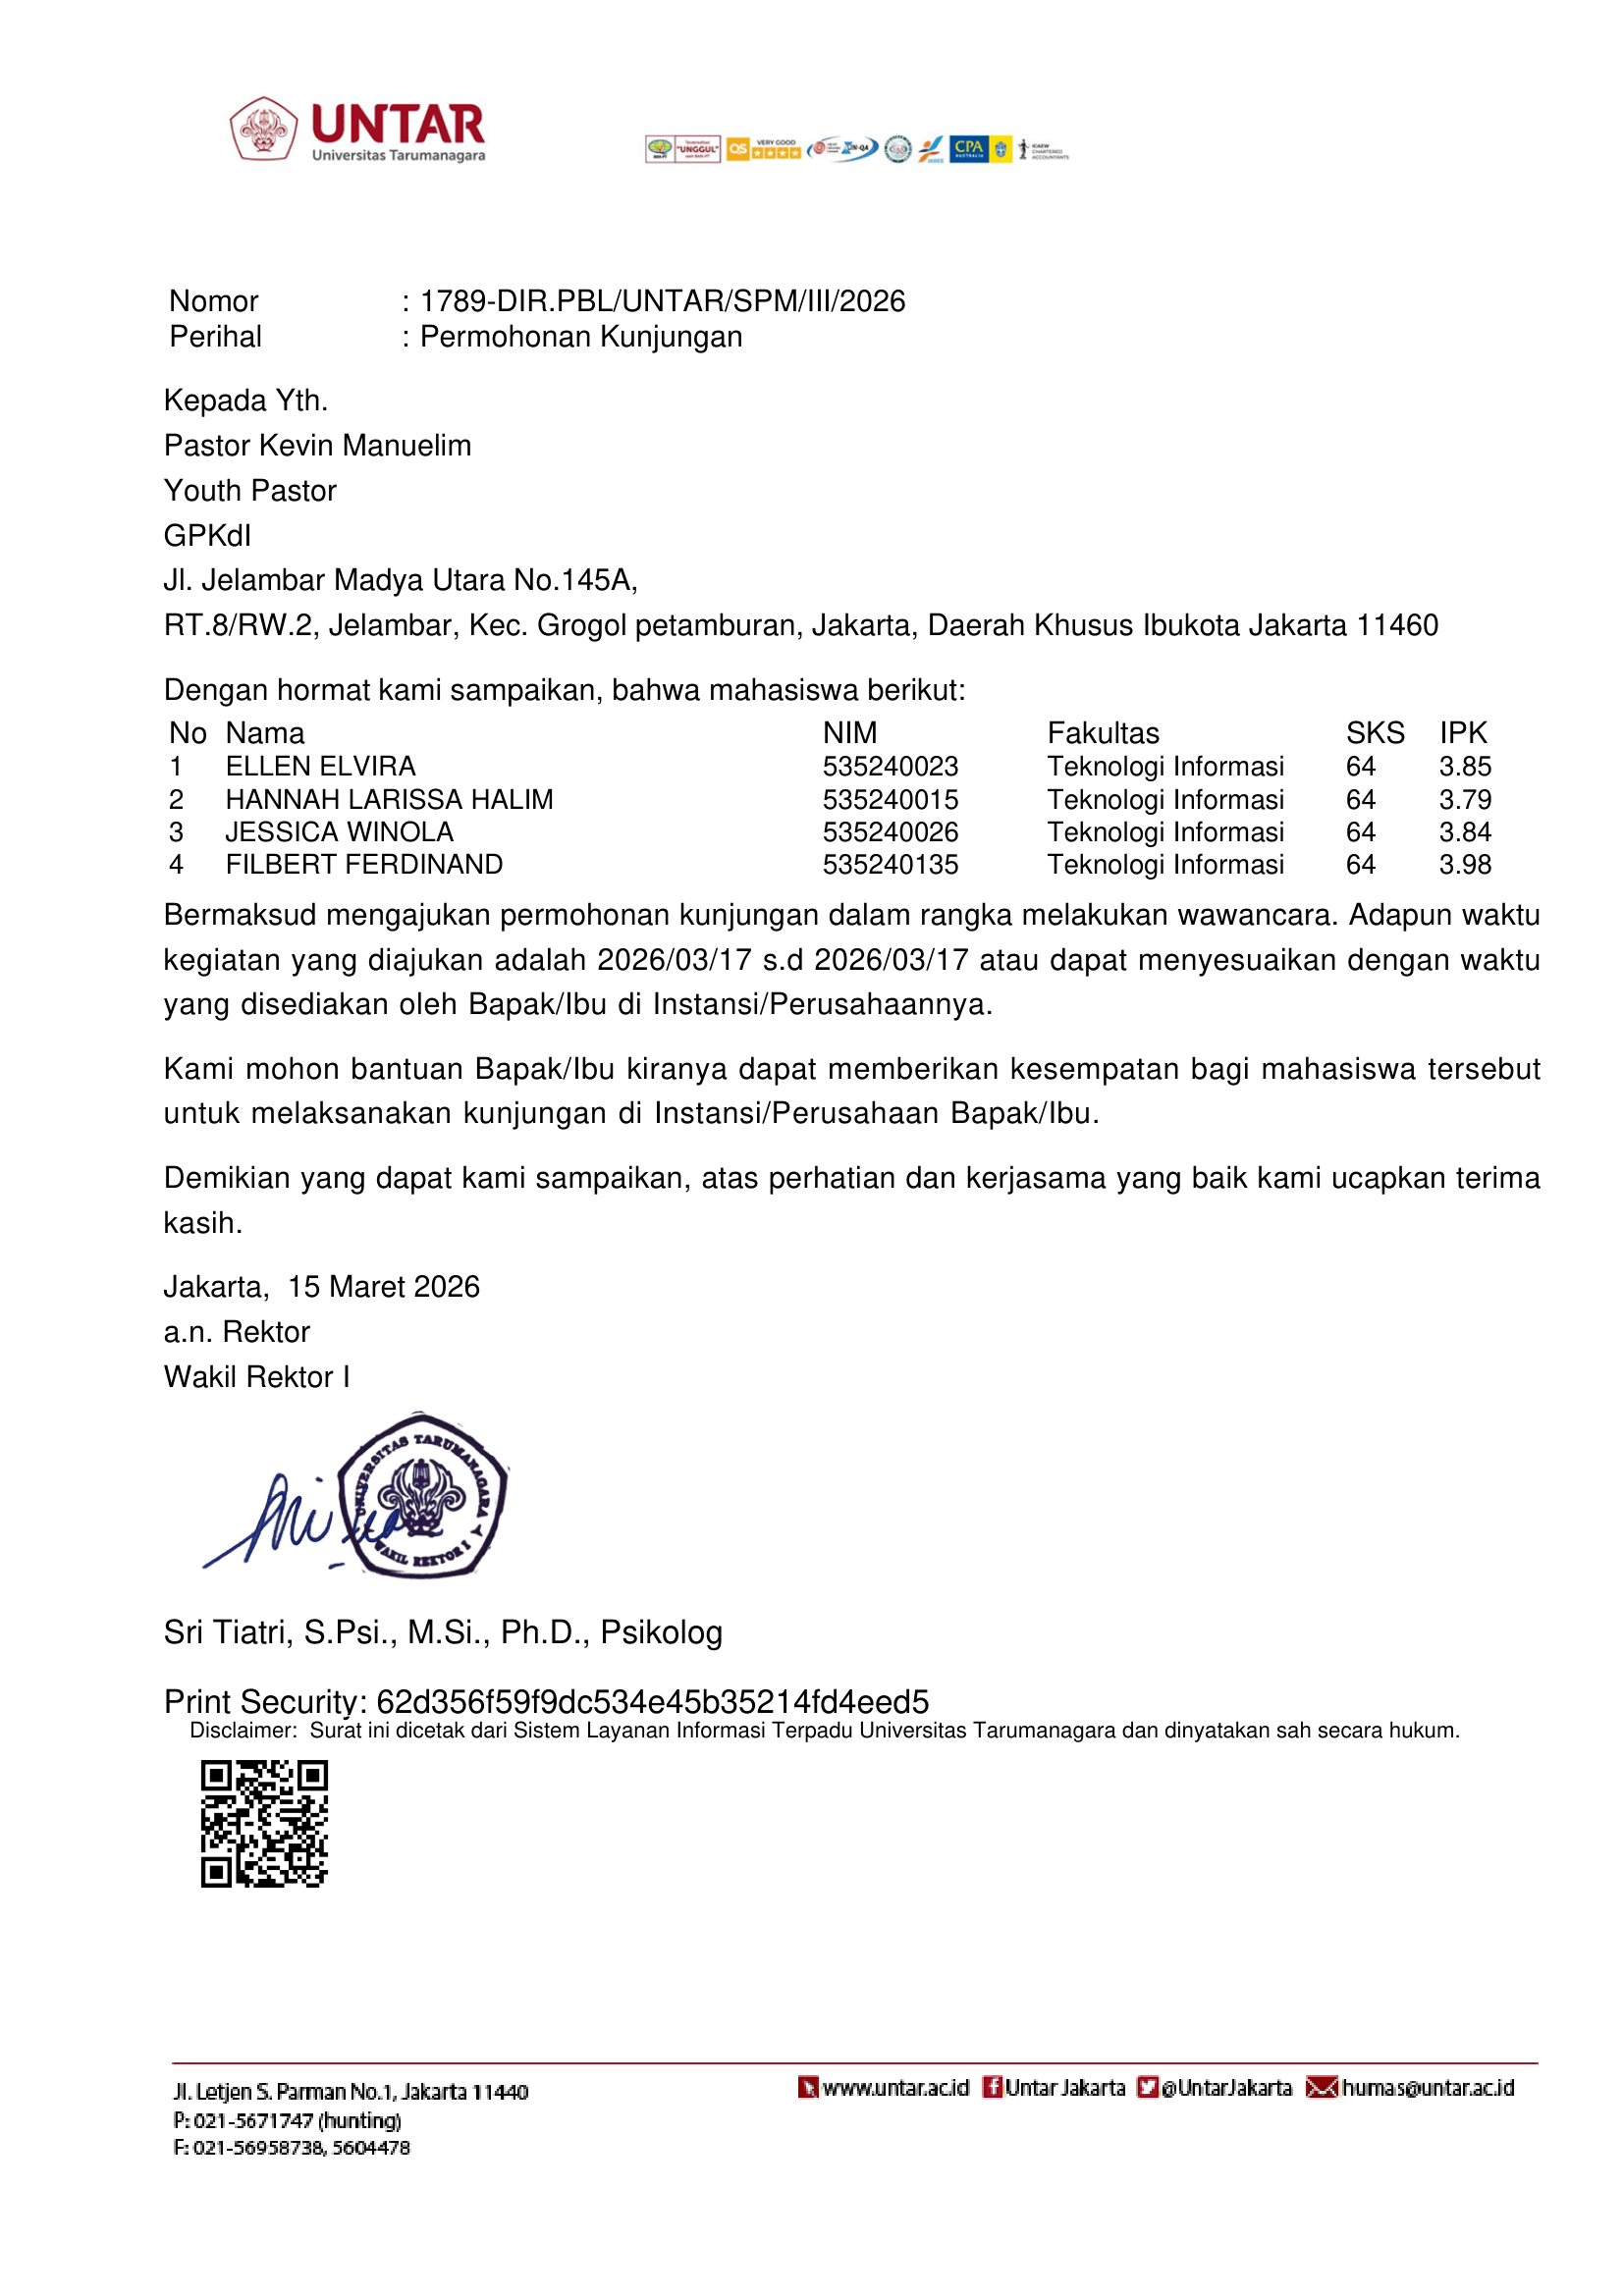
\includegraphics[width = 13cm]{assets/attachments/surat premohonan kunjungan GPKdI .png}
                \captionsetup{labelformat=empty}
                % \caption[Lampiran 2 Surat Permohonan LINTAR]{Lampiran 2 Surat Permohonan LINTAR}
                \label{fig:SuratLINTAR}
            \end{secondfigure}
            \begin{secondfigure}[H]
                \centering
                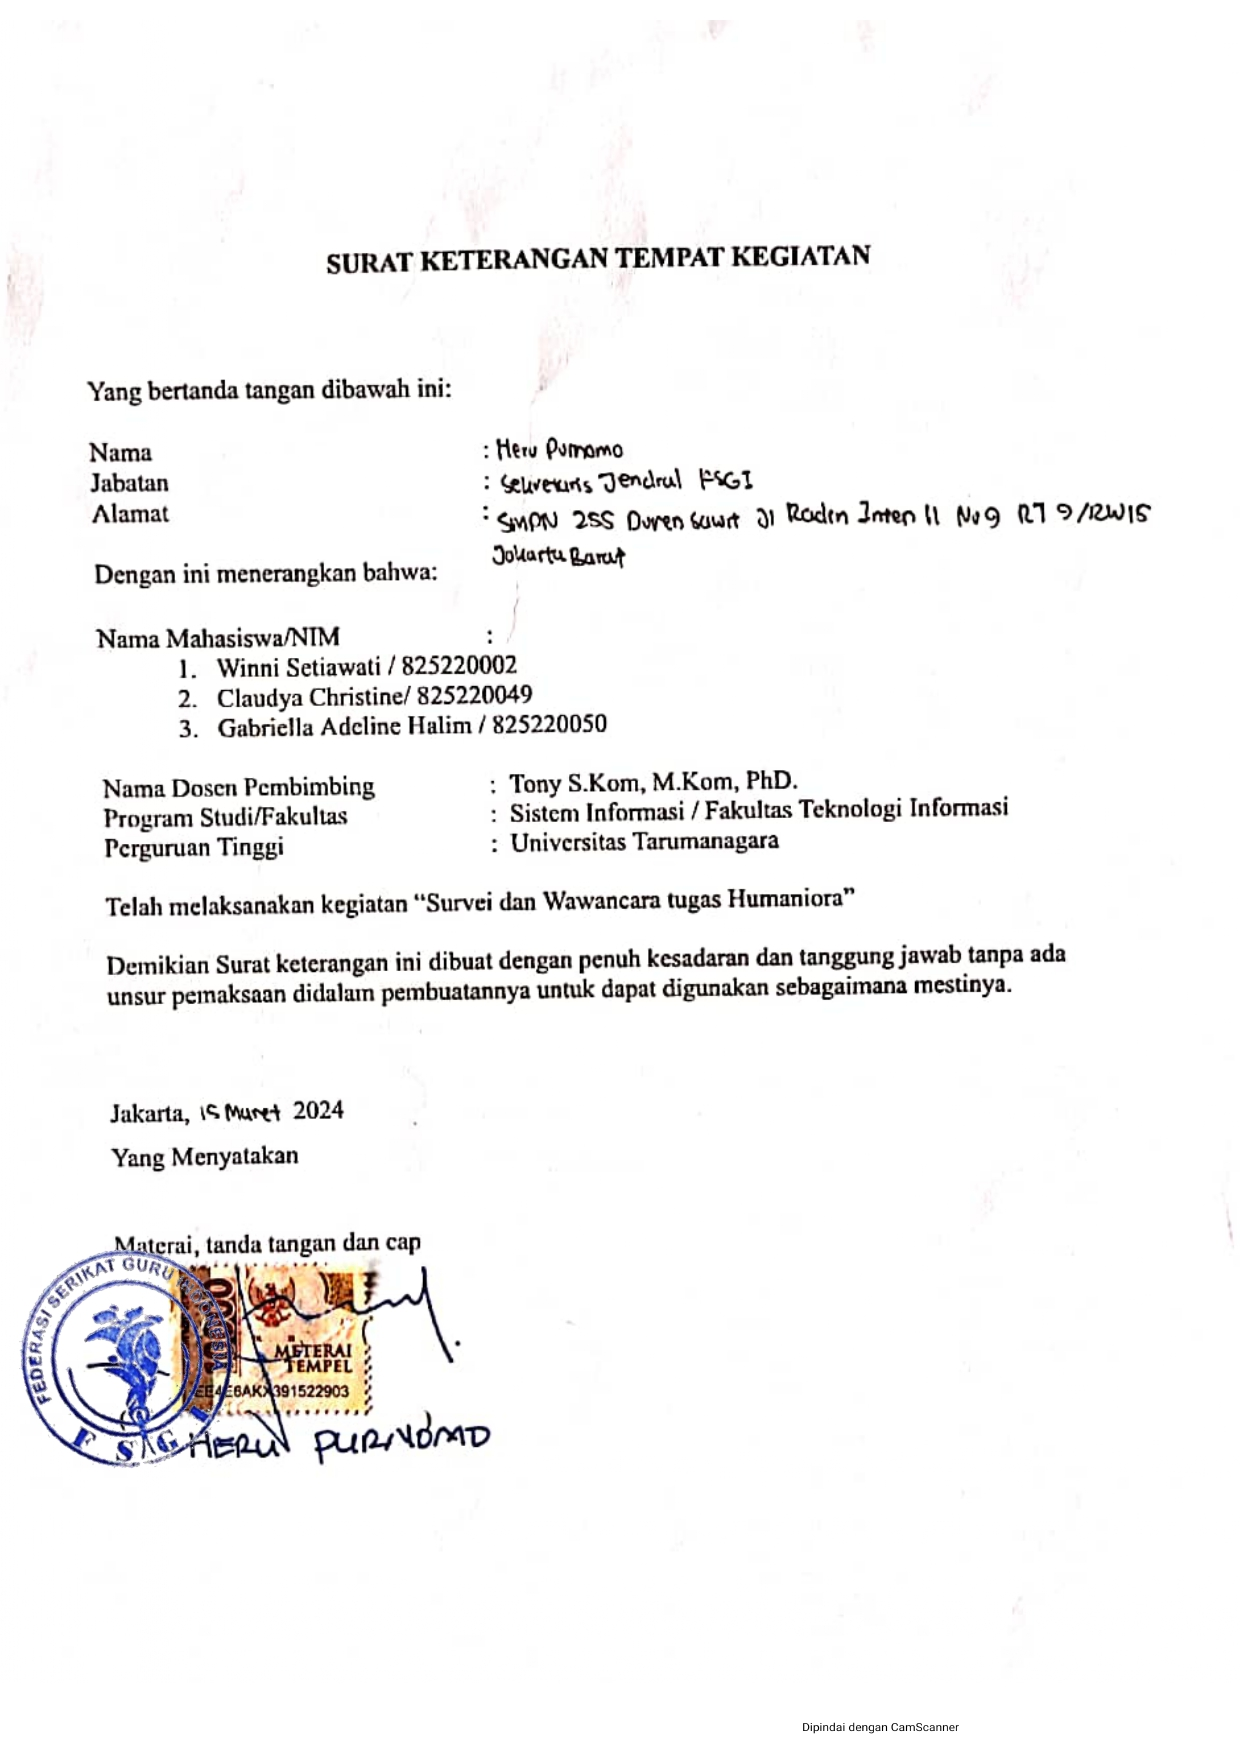
\includegraphics[width = 13cm]{assets/attachments/ttd surat keterangan wawancara_page-0001.jpg}
                \captionsetup{labelformat=empty}
                % \caption[Lampiran 1 Surat Keterangan Tempat Kegiatan]{Lampiran 1 Surat Keterangan Tempat Kegiatan}
                \label{fig:SuratKegiatan}
            \end{secondfigure}
           
\newpage
\label{lampiran2}
\begin{center}
    \addcontentsline{toc}{section}{LAMPIRAN II DOKUMENTASI PELAKSANAAN KEGIATAN}
    \section*{\textbf{LAMPIRAN II DOKUMENTASI PELAKSANAAN KEGIATAN}}
\end{center}
  \begin{secondfigure}[H]
        \centering
        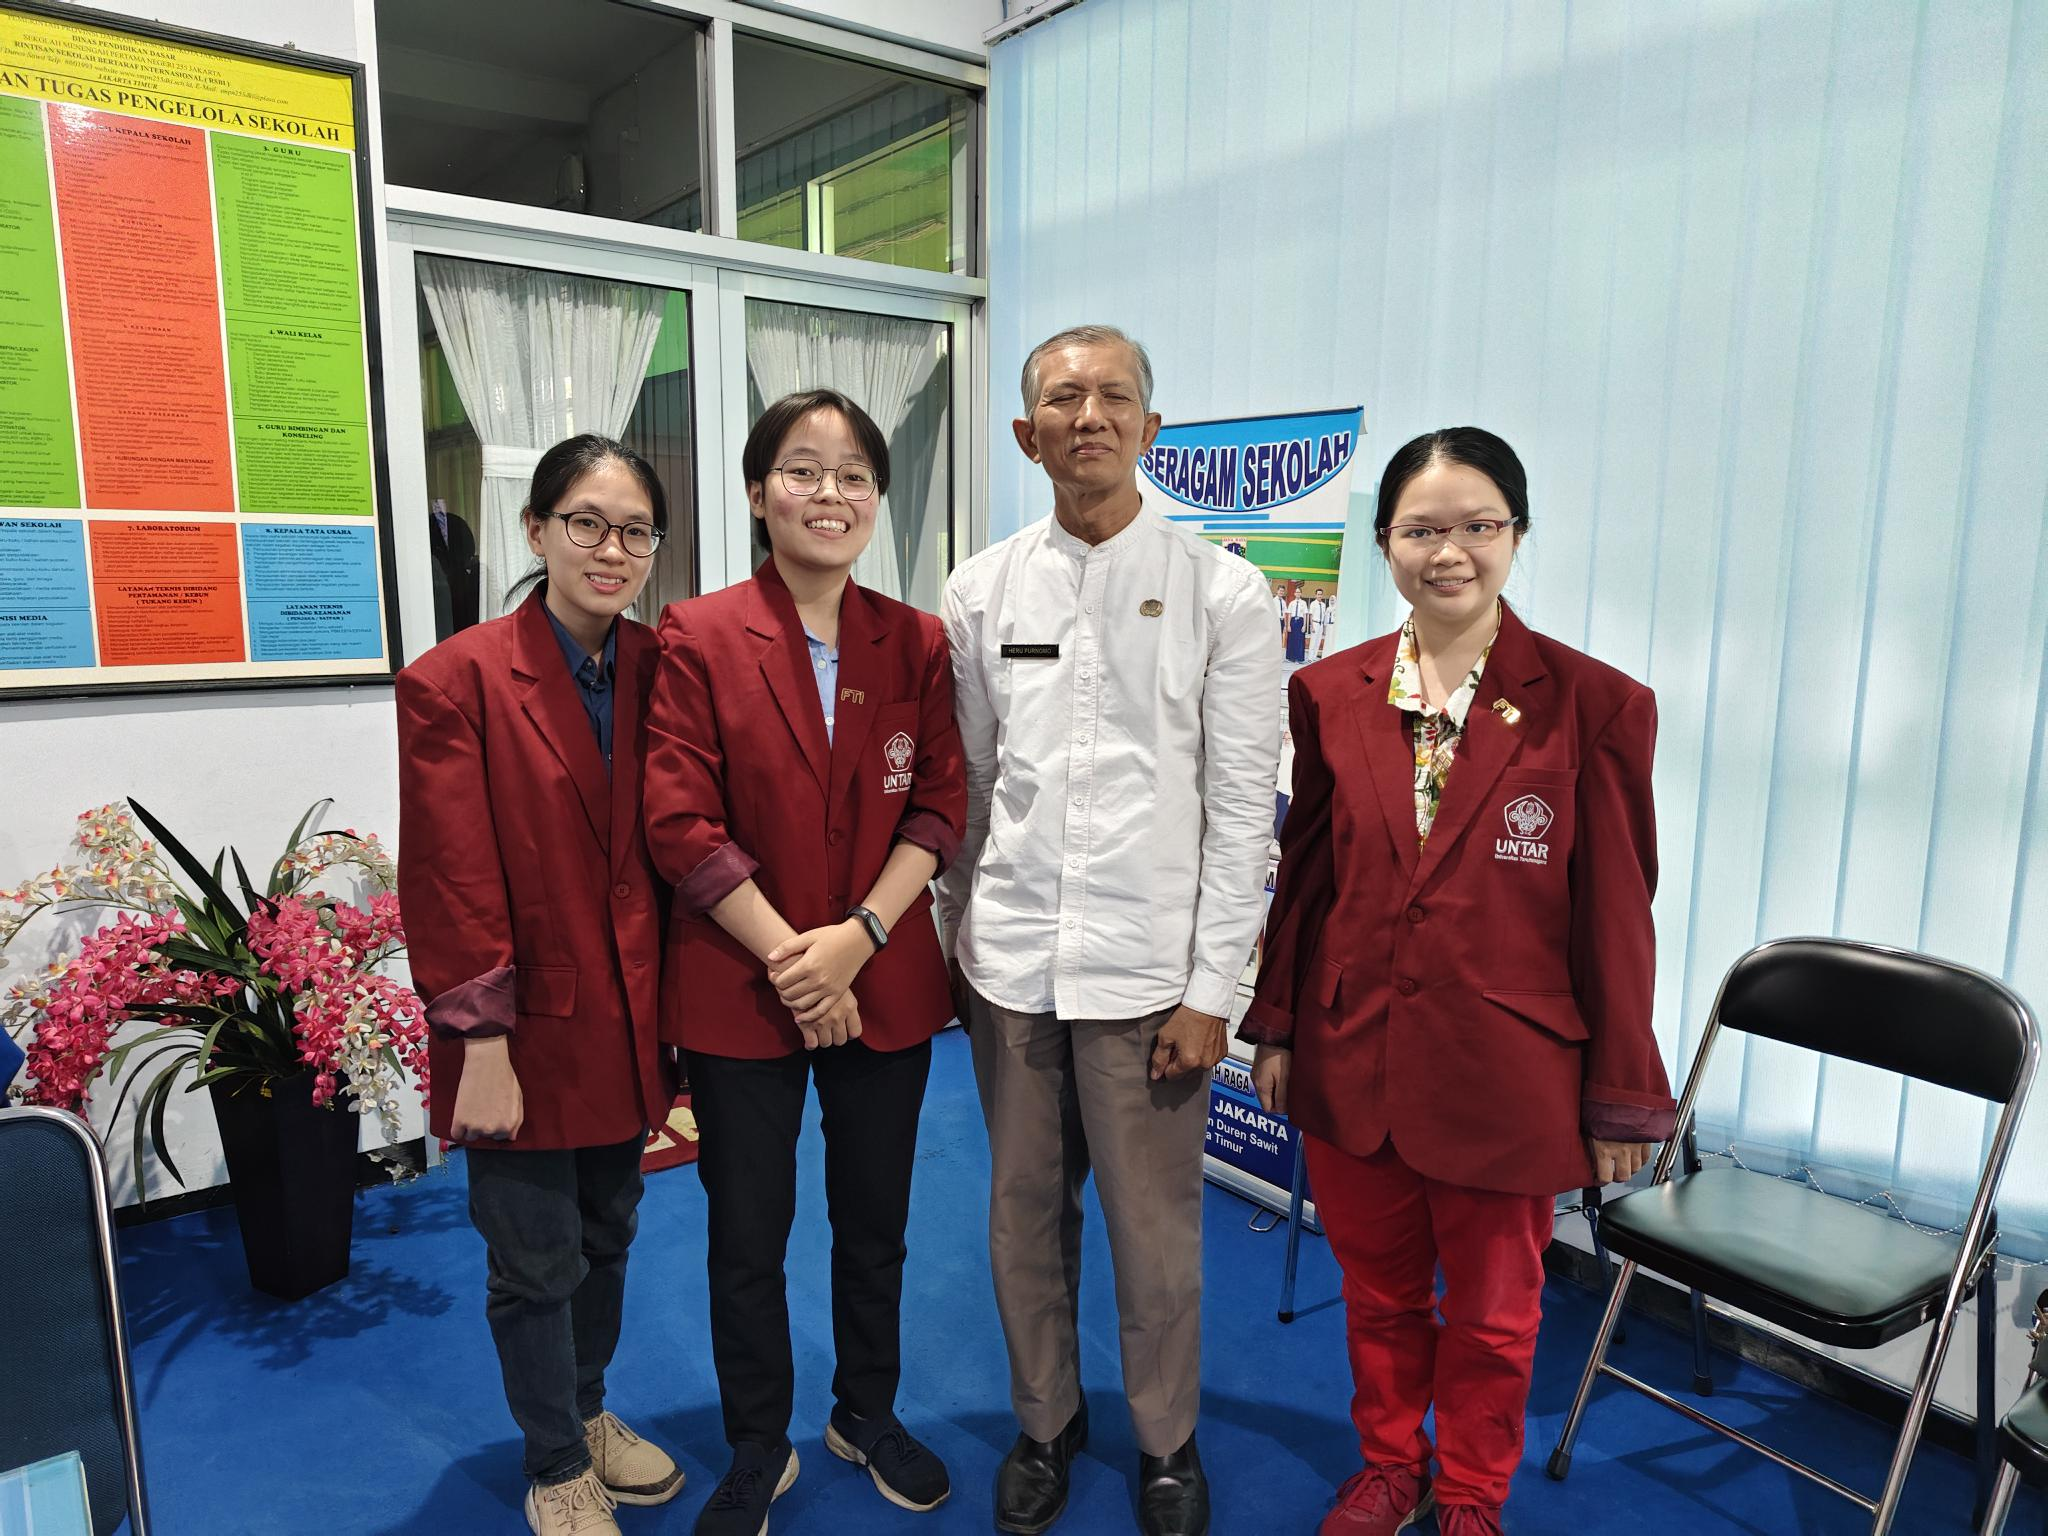
\includegraphics[width = 8cm]{assets/documentation/2 photos added (1).jpeg}
        \captionsetup{labelformat=empty}
        % \caption[Lampiran 3 Wawancara dengan Pak Heru Purnomo Sekretaris Jendral FSGI}
        \label{fig:FotoWawancaraFSGI}
    \end{secondfigure}

    \begin{secondfigure}[H]
        \centering
        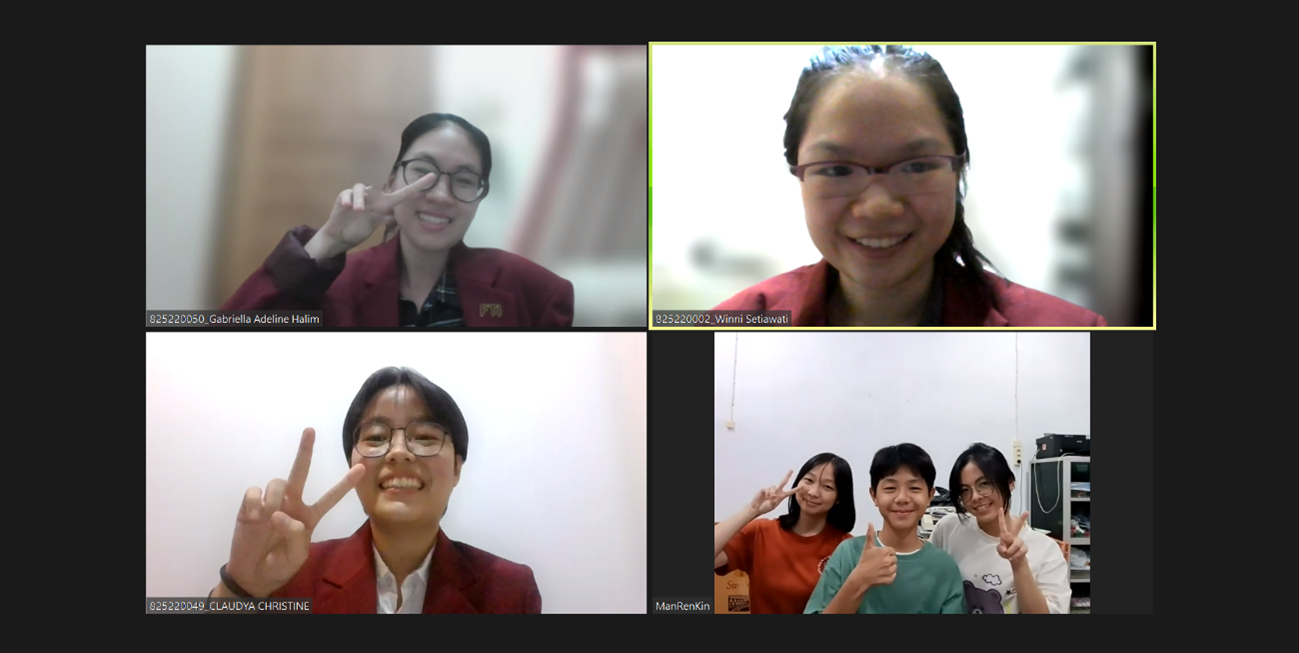
\includegraphics[width = 10cm]{assets/documentation/Picture1wawancarasiswa.png}
        \captionsetup{labelformat=empty}
         % \caption[Lampiran 4 Wawancara dengan siswa]{Lampiran 4 Foto Wawancara dengan siswa}
        \label{fig:FotoWawancarasiswa}
    \end{secondfigure}

    \begin{secondfigure}[H]
        \centering
        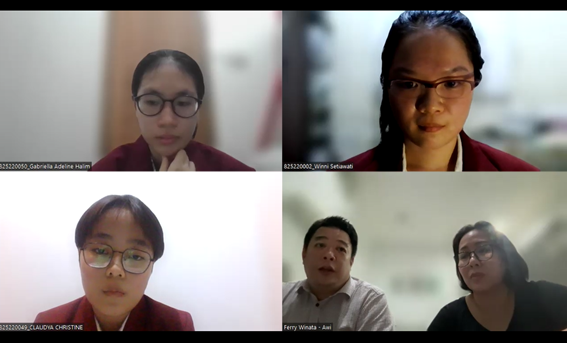
\includegraphics[width = 10cm]{assets/documentation/Picture2wawancaraortu.png}
        \captionsetup{labelformat=empty}
         % \caption[Lampiran 5 Foto wawancara dengan orang tua siswa ]{Lampiran 5 Foto wawancara dengan orang tua siswa }
        \label{fig:FotoWawancaraOrtu}
    \end{secondfigure}

        \begin{minipage}{1\linewidth}
        \begin{minipage}[hb]{0.5\linewidth}
            \begin{secondfigure}[H]
                \centering
                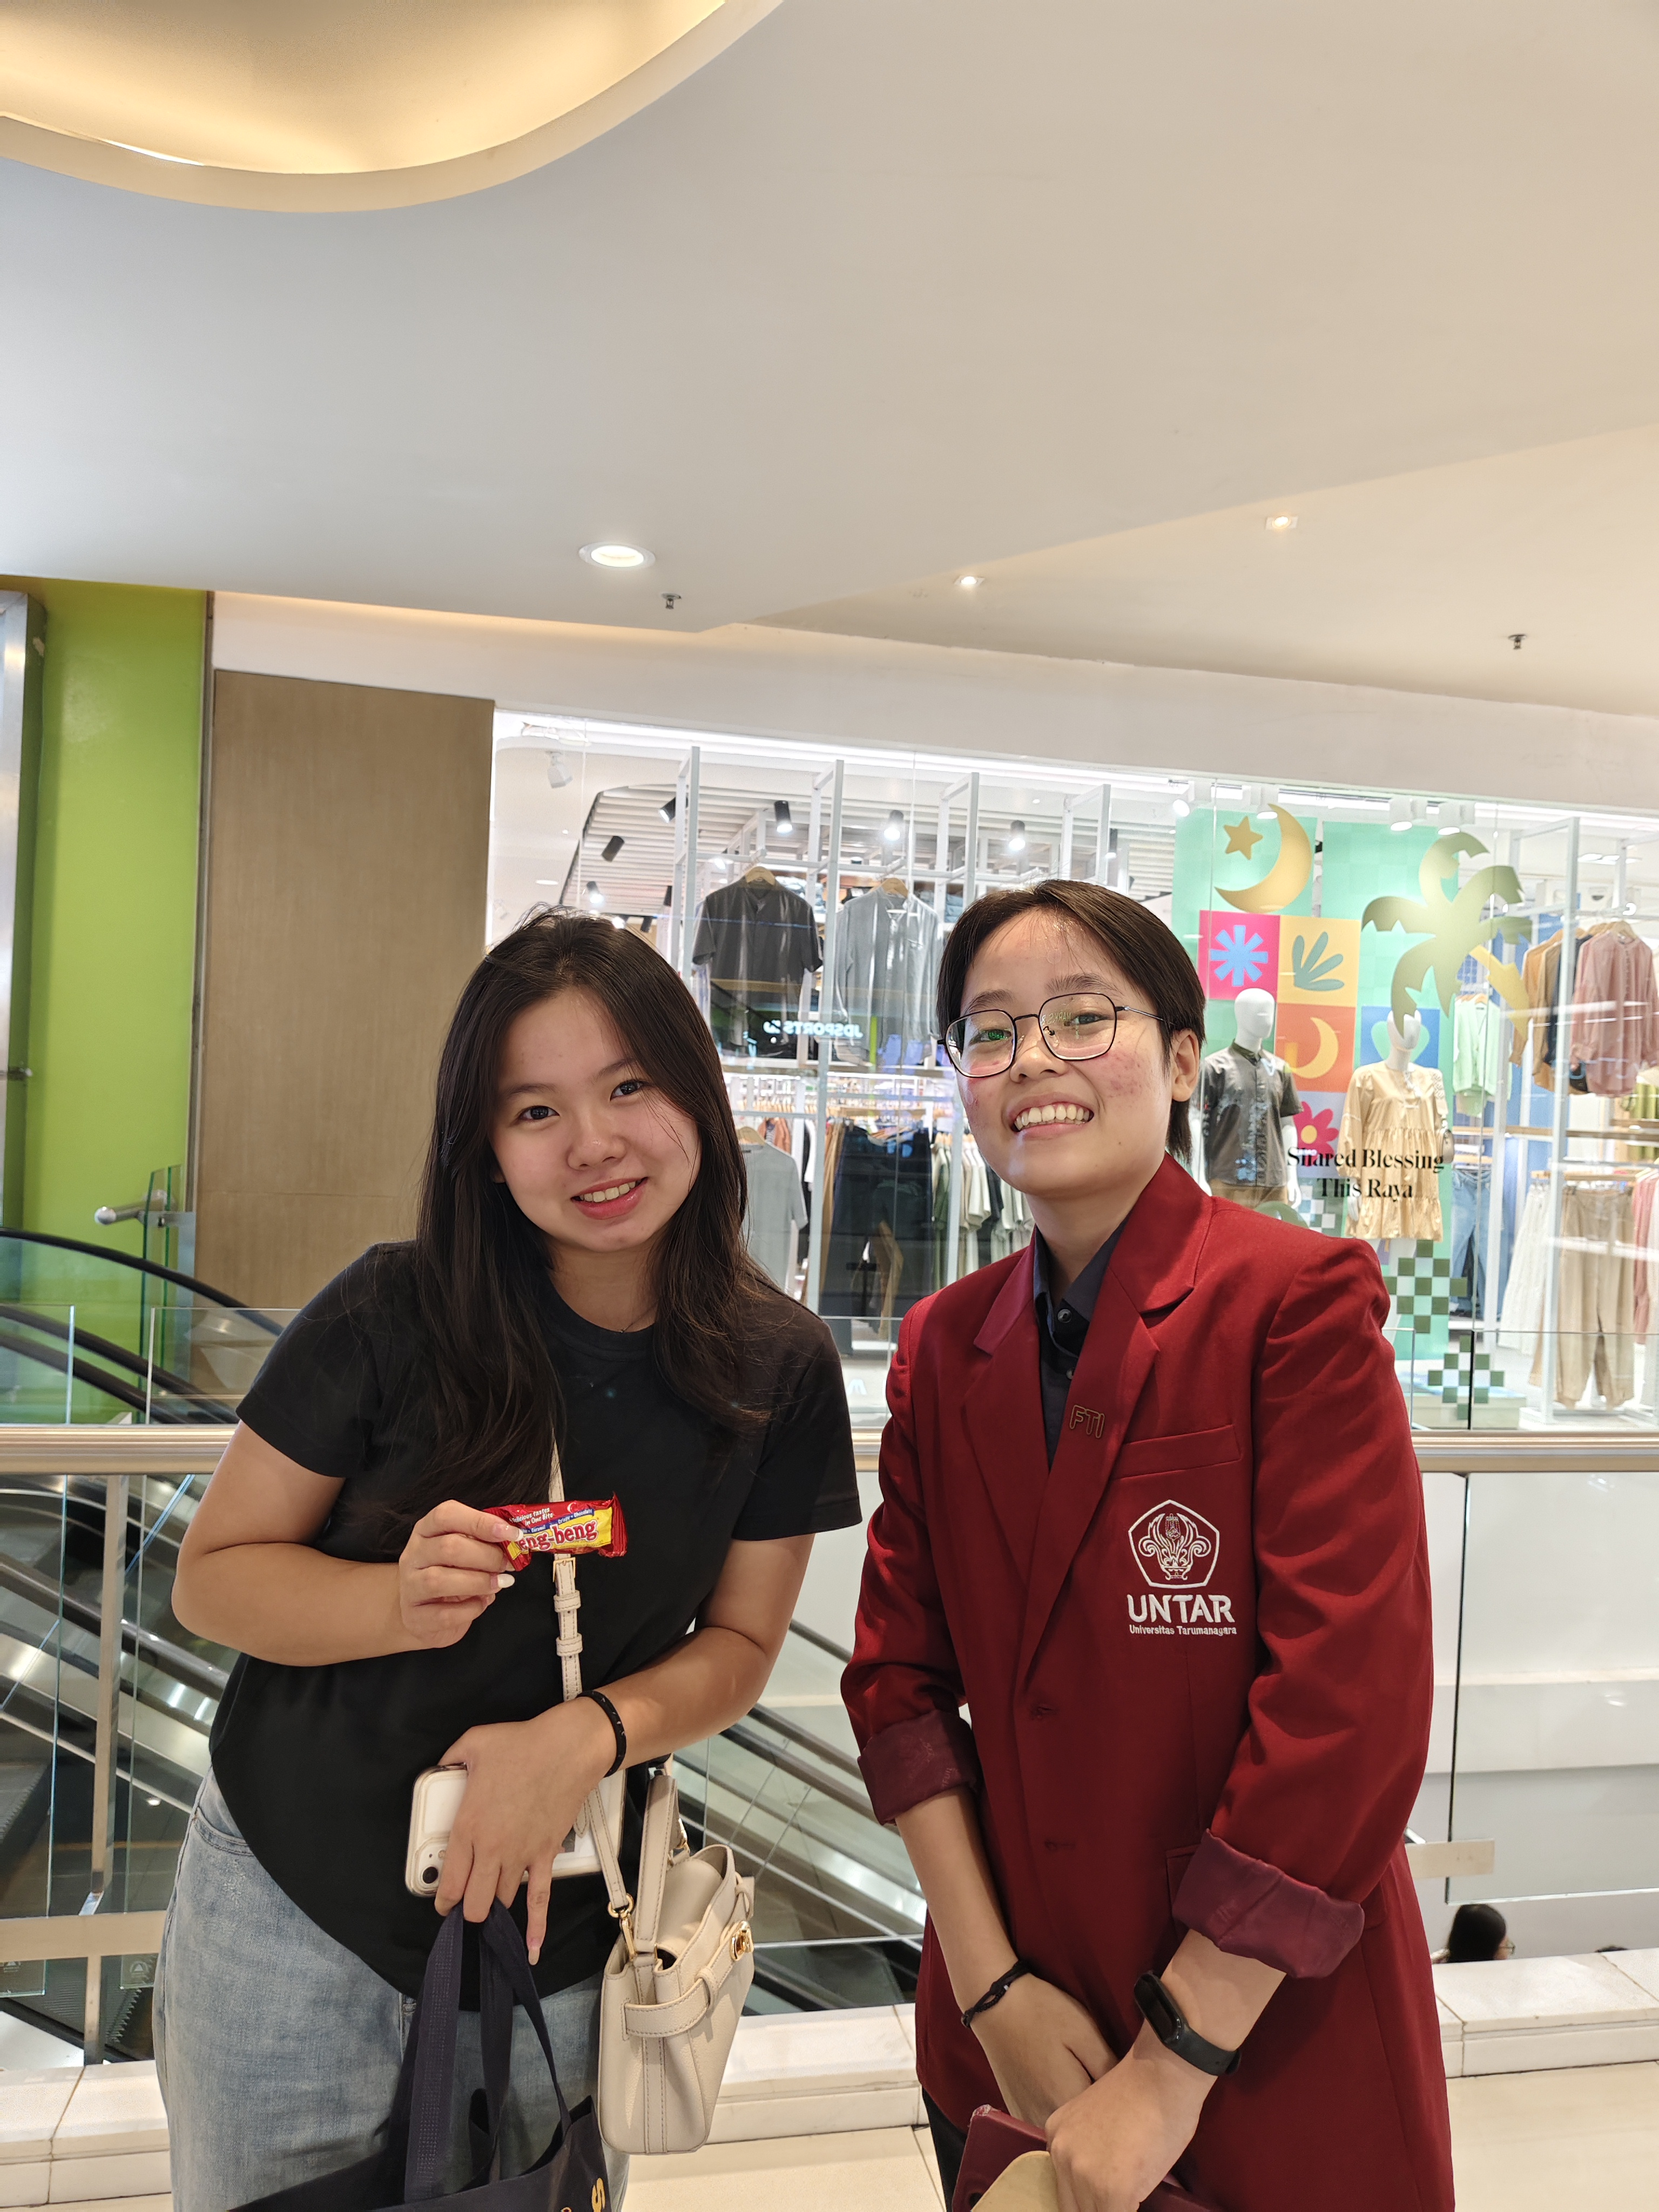
\includegraphics[width = 7cm]{assets/documentation/IMG_20240312_132116.jpg}
                \captionsetup{labelformat=empty}
                 % \caption[Lampiran 6 wawancara masyarakat umum 1]{Lampiran 6 wawancara masyarakat umum 1}
                \label{fig:wawancaramasya1}
            \end{secondfigure}
        \end{minipage}
        \hfill
        \hspace{0.3cm}
        \begin{minipage}[hb]{0.5\linewidth}
                 \begin{secondfigure}[H]
                    \centering
                    \includegraphics[width = 7cm]{assets/documentation/IMG_20240312_134754.jpg}
                    \captionsetup{labelformat=empty}
                     % \caption[Lampiran 7 Foto wawancara masyarakat 2]{Lampiran 7 Foto wawancara masyarakat 2}
                    \label{fig:wawancaramasya2}
                \end{secondfigure}
        \end{minipage}
    \end{minipage}
    
        \begin{secondfigure}[H]
            \centering
            \includegraphics[width = 11cm]{assets/documentation/IMG_20240312_131239.jpg }
            \captionsetup{labelformat=empty}
            % \caption[Lampiran 8 Foto wawancara masyarakat 3}
            \label{fig:wawancaramasya3}
        \end{secondfigure} 

\vspace*{2.cm}



\newpage
\label{lampiran3}
\setcounter{table}{0}

\begin{center}
    \addcontentsline{toc}{section}{LAMPIRAN III DAFTAR PERTANYAAN}
    \section*{\textbf{LAMPIRAN III DAFTAR PERTANYAAN DAN HASIL JAWABAN KUESIONER}}
\end{center}

\hspace{5cm}

\begin{table}[h]

\captionsetup{labelformat=empty}
\caption[Persentase sebaran jawaban kuesioner berdasarkan kategori pertanyaan pengetahuan responden terhadap pengertian, penyebab, dampak, tata laksana \textit{cyberbullying} ada anak usia sekolah]{Tabel \ref{tab:TabelhasilkuesionerX1} Persentase sebaran jawaban kuesioner berdasarkan kategori pertanyaan pengetahuan responden terhadap pengertian, penyebab, dampak, tata laksana \textit{cyberbullying} ada anak usia sekolah}
\label{tab:TabelhasilkuesionerX1}

\begin{tabular}{ |p{1.4cm}|p{5.4cm}|p{1.3cm}|p{1cm}|p{1cm}|p{1cm}|p{1cm}| } 
\hline
\centering \textbf{Kategori Variabel} & \centering \textbf{Butir Pertanyaan} & \centering \textbf{Sangat Tidak Setuju (\%)} & \centering \textbf{Tidak Setuju (\%)} & \centering \textbf{Netral (\%)} & \centering \textbf{Setuju (\%)} &  \textbf{\centering Sangat Setuju (\%)} \\
\hline
\multicolumn{7}{|c|}{X1 : Pengetahuan responden terhadap pengertian, penyebab, dampak, tata laksana \textit{cyberbullying} }\\
\multicolumn{7}{|c|}{ada anak usia sekolah} \\
\hline
X1 & Saya mengetahui apa itu \textit{cyberbullying}. & 12,2 & 3,6 & 11,5 & 43,5 & 29,5 \\
\hline
X1 & Saya mengetahui penyebab \textit{cyberbullying} pada siswa bisa terjadi. & 7,2 & 3,6 & 15,1 & 54,7 & 19,4 \\
\hline
X1 & Saya mengetahui dampak yang dihasilkan oleh \textit{cyberbullying} terhadap korban maupun pelaku. & 7,9 & 2,9 & 8,6 & 52,5 & 28,1 \\
\hline
X1 & \textit{Cyberbullying} merupakan kelanjutan dari \textit{bullying} konvensional dengan menggunakan media sosial/alat media \textit{virtual}. & 7,9 & 2,2 & 10,8 & 51,1 & 28,1 \\
\hline
X1 & Saya sering melihat atau mendengar kasus \textit{cyberbullying} di lingkungan sekolah atau masyarakat. & 7,2 & 8,6 & 17,3 & 46 & 20,9 \\
\hline
X1 & Saya mengetahui tindakan yang harus saya ambil ketika seorang siswa sedang menjadi korban \textit{cyberbullying}. & 2,2 & 7,2 & 25,2 & 51,8 & 13,7 \\
\hline 

\end{tabular}
\end{table}

\begin{table}[h]

\captionsetup{labelformat=empty}
\caption[Persentase sebaran jawaban kuesioner berdasarkan kategori pertanyaan tingkat kepuasan responden terhadap upaya sekolah dan mengerti pentingnya kolaborasi sosial berjenjang]{Tabel \ref{tab:TabelhasilkuesionerX2} Persentase sebaran jawaban kuesioner berdasarkan kategori pertanyaan tingkat kepuasan responden terhadap upaya sekolah dan mengerti pentingnya kolaborasi sosial berjenjang}
\label{tab:TabelhasilkuesionerX2}
\begin{tabular}{ |p{1.4cm}|p{5.4cm}|p{1.3cm}|p{1cm}|p{1cm}|p{1cm}|p{1cm}| } 
\hline
\centering \textbf{Kategori Variabel} & \centering \textbf{Butir Pertanyaan} & \centering \textbf{Sangat Tidak Setuju (\%)} & \centering \textbf{Tidak Setuju (\%)} & \centering \textbf{Netral (\%)} & \centering \textbf{Setuju (\%)} &  \textbf{\centering Sangat Setuju (\%)} \\
\hline
\multicolumn{7}{|c|}{X2 : Tingkat kepuasan responden terhadap upaya sekolah dan mengerti pentingnya kolaborasi } \\
\multicolumn{7}{|c|}{sosial berjenjang } \\

\hline
X2 & Saya mengetahui tindakan yang harus saya ambil ketika seorang siswa sedang menjadi korban \textit{cyberbullying}. & 6,5 & 26,6 & 33,1 & 23,7 & 10,1 \\
\hline
X2 & Pihak sekolah telah mengupayakan untuk meminimalisir kejadian \textit{cyberbullying} siswa di lingkungan sekolah berupa kebijakan memasukkan ponsel siswa ke dalam \textit{box} selama tidak dibutuhkan saat pelajaran. Menurut saya kebijakan tersebut baik untuk diterapkan. & 5,8 & 11,5 & 23,7 & 44,6 & 14,4 \\
\hline
X2 & Menurut saya penyamaan persepsi mengenai pencegahan \textit{cyberbullying} memerlukan kolaborasi antara sekolah, masyarakat, pemerintah, dan pihak terkait lainnya. & 0 & 2,2 & 7,2 & 46,8 & 43,9 \\
\hline
X2 & Saya merasa kolaborasi antar sekolah, masyarakat, pemerintah, dan pihak terkait lainnya untuk mencegah dan menganggulangi \textit{cyberbullying} pada anak sekolah sudah baik. & 2,9 & 28,8 & 36,7 & 24,5 & 7,2 \\
\hline
X2 & Menurut saya sosialisasi kepada orang tua dan anak-anak didik mengenai kebijakan penggunaan ponsel yang terhubung internet di lingkungan sekolah sudah baik. & 3,6 & 23 & 34,5 & 29,5 & 9,4 \\
\hline
X2 & Saya merasa literasi \textit{digital} dapat mengurangi dampak negatif penggunaan teknologi \textit{digital} pada siswa. & 0 & 6,5 & 29,5 & 46 & 18 \\
\hline
\end{tabular}
\end{table}

\begin{table}[h]

\captionsetup{labelformat=empty}
\caption[Persentase sebaran jawaban kuesioner berdasarkan kategori pertanyaan kesediaan responden melakukan perilaku bela negara untuk mencegah terjadinya \textit{cyberbullying} pada anak tingkat sekolah]{Tabel \ref{tab:TabelhasilkuesionerX3} Persentase sebaran jawaban kuesioner berdasarkan kategori pertanyaan kesediaan responden melakukan perilaku bela negara untuk mencegah terjadinya \textit{cyberbullying} pada anak tingkat sekolah}
\label{tab:TabelhasilkuesionerX3}
\begin{tabular}{ |p{1.4cm}|p{5.4cm}|p{1.3cm}|p{1cm}|p{1cm}|p{1cm}|p{1cm}| } 
\hline
\centering \textbf{Kategori Variabel} & \centering \textbf{Butir Pertanyaan} & \centering \textbf{Sangat Tidak Setuju (\%)} & \centering \textbf{Tidak Setuju (\%)} & \centering \textbf{Netral (\%)} & \centering \textbf{Setuju (\%)} &  \textbf{\centering Sangat Setuju (\%)} \\
\hline
\multicolumn{7}{|c|}{X3 : Kesediaan responden melakukan perilaku bela negara untuk mencegah terjadinya } \\
\multicolumn{7}{|c|}{\textit{cyberbullying} pada anak tingkat sekolah} \\
\hline
X3 & Bila saya diberikan kesempatan untuk berkolaborasi dengan sekolah, pemerintah, atau pihak terkait lainnya untuk mencegah dan menanggulangi \textit{cyberbullying} pada siswa saya bersedia untuk turun tangan secara langsung. & 1,4 & 5 & 31,7 & 51,8 & 10,1 \\
\hline
X3 & Saya merasa sikap bela negara dapat menjadi solusi untuk mencegah terjadinya \textit{cyberbullying}. & 0 & 5 & 25,9 & 51,1 & 18 \\
\hline
X3 & Saya merasa masyarakat memiliki peran penting dalam pencegahan dan penanganan \textit{cyberbullying}. & 7 & 2,2 & 10,1 & 51,8 & 35,3 \\
\hline
\end{tabular}
\end{table}
